\chapter{Energy Harvesting in IoT}
In general, finite battery capacity calls for a tradeoff between performance and lifetime of IoT devices, which is a major challenge in the IoT domain. Energy harvesting is a promising solution to this challenge, as it can provide a continuous and sustainable energy source for IoT devices. In this chapter, we provide an overview of energy harvesting in IoT, including the energy sources, energy harvesting techniques, and the challenges and opportunities in this area.

\section{Introduction and definitions}
Energy harvesting converts energy from one form to another.
If the harvested energy source
is large and periodically/continuously available, a device can last ``forever''.
This approach also allows to tune the device parameters for a better performance, since it removes the constraint of lifetime.

Note that the energy production varies with time and on environmental conditions; 
this is an aspect typically out of the control of the designer.

\begin{definition}[Energy Source]
   Source of energy to be harvested
   \note{Sun, wind, etc\dots}
\end{definition}

\begin{definition}
   [Harvesting source] 
   Any available harvesting technology, (solar cells, wind turbines, piezo-electric harvesters etc\dots) that extracts energy from the environment.
\end{definition}

\begin{definition}
   [Load]
   Consumption of energy in a device due to its activities
   \begin{itemize}
      \item A device has many subsystems
      (processor/memory, radio, storage,
      transducers/ADC), each with its own states and
      consumption
      \item The load varies over time:
      depends on the specific activities the device is
      executing at a time
   \end{itemize}
\end{definition}

\begin{definition}
   [Harvesting System]

   \begin{itemize}
      \item a system that supports a variable load from a variable energy-harvesting source
      \item \dots also when the instantaneous power supply levels from the harvesting source do not match the load.
   \end{itemize}
\end{definition}

\subsection{Takeaway}
In theory, there are two main approaches:
\begin{enumerate}
   \item adapt the load to the actual energy supply
   \item use an energy buffer
   \note{i.e. a rechargeable battery or a
   supercapacitor}
\end{enumerate}

However, in practice neither of these two approaches may be sufficient, since the load cannot be reduced arbirarily, and the buffer is not ideal (no infinite storage and eventually energy leaks).
\newpage
\section{Harvesting Architectures}
\subsection{Harvest-use}
\begin{paracol}{2}

   In this architecture energy is harvested just-in-time for use.\\
   The power output has to be above the minimum operating point (else the device turns OFF), 
   but note that this might leads abrupt variations to cause the device to oscillate between ON and OFF states.
   
   The problem is that a device may suffer from ``Alzheimer's disease'', i.e. it forgets what it was doing before turning OFF, since the content of the RAM is lost.
   \note{This is an issue currently being addressed by researchers.}
   
   \switchcolumn
   
   \begin{figure}[htbp]
      \centering
      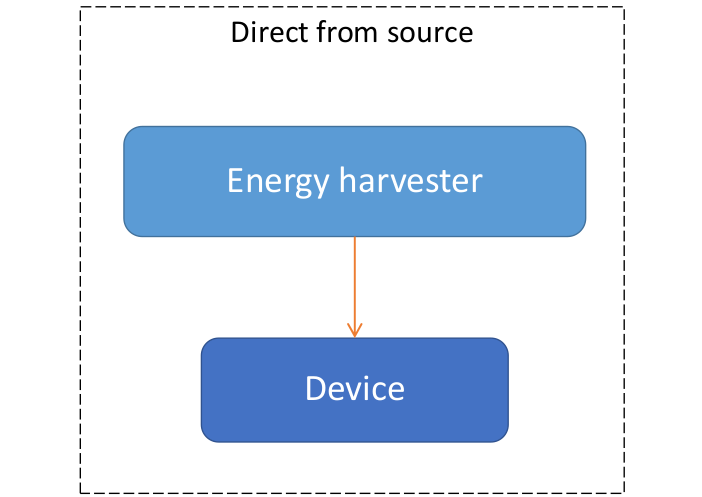
\includegraphics[width=0.45\columnwidth]{images/harvestuse1.png}
      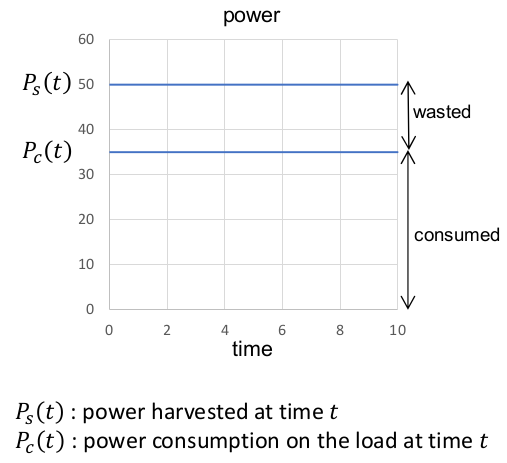
\includegraphics[width=0.45\columnwidth]{images/harvestuse2.png}
      \caption{Harvest use schema}
      \label{fig:harvestuse}
   \end{figure}
\end{paracol}

The energy harvested, but not required by the device functioning is \textbf{wasted}.

TODO modeling

\subsection{Harvest-store-use}
\begin{paracol}{2}
   \colfill
   Energy is harvested whenever
   possible and stored for future
   use.\\
   Residual energy is stored and it
   is used later when either there
   are no harvesting opportunities
   or the device tasks require more
   energy.
   \colfill
   \switchcolumn
   \begin{figure}[htbp]
      \centering
      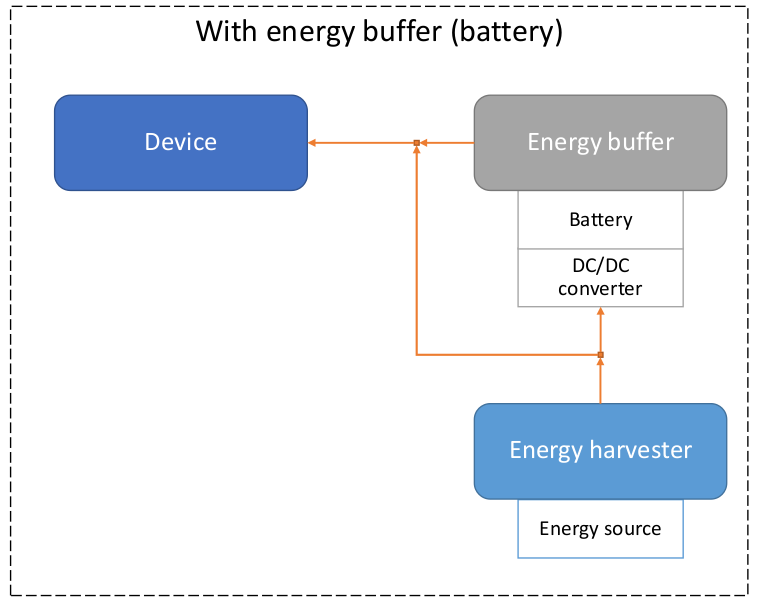
\includegraphics{images/harveststoreuse1.png}
      \caption{Harvest-store-use schema}
      \label{fig:harveststoreuse1}
   \end{figure}
\end{paracol}

\begin{paracol}{2}
   
   We assume for the moment that the energy buffer is ideal, i.e. it can store an infinite amount of energy, it does not leak, and has a charging efficiency $\eta = 1$.\\
   Under such assumptions the device can operate at any time if, for every time interval $(0,T]$
   \begin{align*}
      P_s(t) & \quad & \textit{power harvested at time t}\\
      P_c(t) & \quad & \textit{power consumed on the load at time t}\\
      B_0 & \quad & \textit{initial energy in the buffer}
   \end{align*}
   \[
      \int_0^T P_c(t)dt \leq \int_0^T P_s(t)dt + B_0 \quad \forall T \in (0, \infty)
      \]
      
      \switchcolumn
      \begin{figure}[htbp]
         \centering
         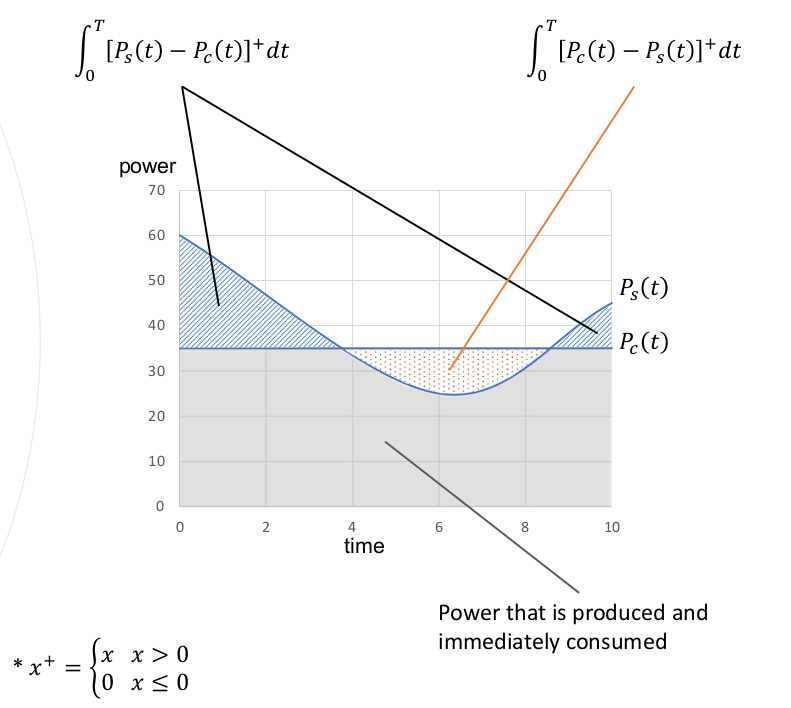
\includegraphics{images/harveststoreuse2.png}
         \caption{Harvest-store-use modeling schema}
         \label{fig:harveststoreuse2}
      \end{figure}
   \end{paracol}

\subsection{Harvest-store-use with a non-ideal buffer}
We need to introduce other symbols
\begin{align*}
   B_{max} & \quad & \textit{maximum battery capacity (energy buffer size)}\\
   B_{t} & \quad & \textit{battery charge at time t}\\
   P_{leak}(t) & \quad & \textit{be the leakage power of the battery at time t}\\
   \eta < 1 & \quad & \textit{be the charging efficiency of the battery}\\
   P_s(t) & \quad & \textit{power harvested at time t}\\
   P_c(t) & \quad & \textit{load at time t}\\
   B_0 & \quad & \textit{initial charge of the buffer}\\
   x^+ = \begin{cases}
      x & \text{if } x > 0\\
      0 & \text{otherwise}
   \end{cases} 
   & \quad & x^+\textit{is a ``rectifier function''}
\end{align*}

\[
   B_T = B_0 + \eta\int_0^T[P_s(t) - P_c(t)]^+dt - \int_0^T[P_c(t) - P_s(t)]^+dt - \int_0^T P_{leak}(t)dt   \quad \forall T \in (0, \infty]
\]

\subsection{Exercise}
\begin{figure}[htbp]
   \centering
   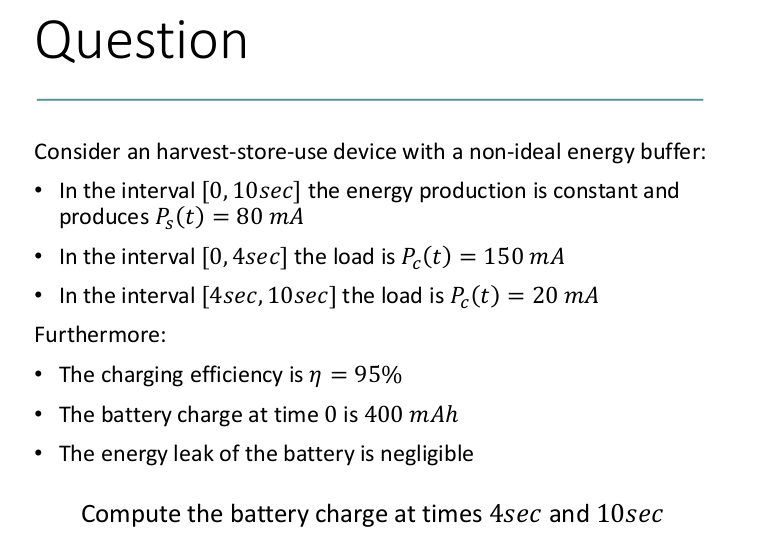
\includegraphics{images/harveststoreuse_question.png}
   \label{fig:harveststoreuse_question}
\end{figure}
\begin{equation}   
\begin{split}
   \textit{Conversion from mAs to mAh} & 3600 mAs = 1 mAh \\
   \\
   400mAh + \hcancel[red]{0.95\times (80-150=-70)\times 4} - 4\times (150-80=70)mAs\\
   400mAh - 280mAs/3600 = 399.92mAh\\
   \textit{\ul{Battery charge at time 4 sec}} = 399.92mAh\\
   \\
   399.92mAh+ 0.95\times (80-20=60)\times 6/3600mAh - \hcancel[red]{6\times (20-60=-40)}\\
   \textit{\ul{Battery charge at time 10 sec}} = 400.02mAh 
\end{split}
\end{equation}

\section{Energy sources classification}
\begin{itemize}
   \item \textbf{Fully controllable} energy sources can provide harvestable energy whenever required.
   \note{Example self-power flashlights: the user may shake to generate energy whenever needed}
   \item \textbf{Partially controllable} energy sources may be influenced by the system design, but the result may not be deterministic
   \note{e.g. RF energy source installed in a room and RFID’s may extract energy from it. However,
   the energy produced at a node depends on RF propagation in the room that cannot be fully
   controlled}
   \item \textbf{Non-controllable} energy sources cannot be activated on demand.
   In these cases the energy must be harvested whenever available.
   \note{e.g. wind, sun, etc\dots}
   \begin{itemize}
      \item \textbf{Predictable} energy sources are those for which there exist reliable models
      that forecast the energy availability.
      \note{e.g. Sun cannot be controlled but it can be predicted (to some extent).
      Day/night production, summer/winter, weather forecasts, \dots}
      \item \textbf{Unpredictable}
      energy sources are those for which there not exist reliable models that forecast the energy availability
      \note{e.g. vibration due to sources for which there are no models available (earthquakes etc\dots)}
   \end{itemize}
\end{itemize}

\begin{figure}[htbp]
   \centering
   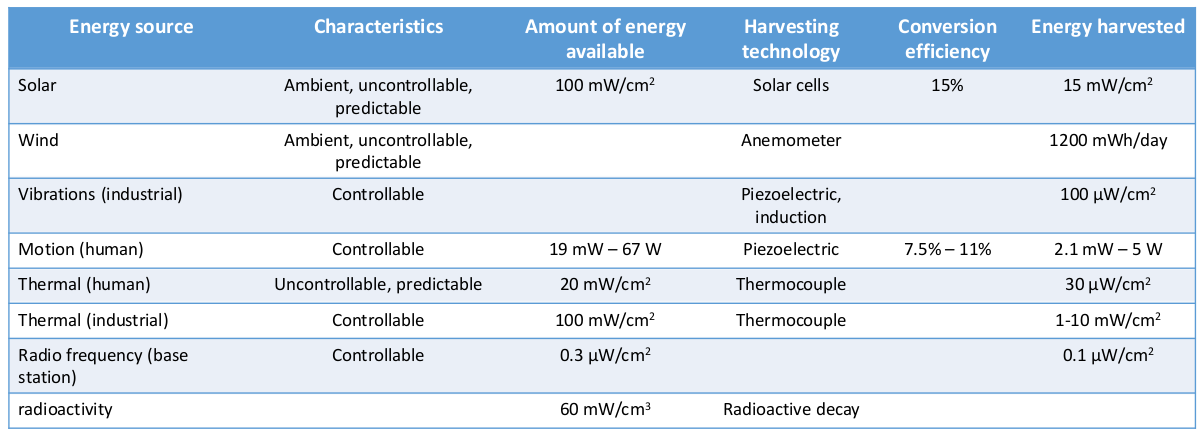
\includegraphics{images/energysources.png}
   \caption{Energy sources summary}
   \label{fig:energysources}
\end{figure}
\note{Fun fact: the efficiency of the plants' photosynthesis is around $10-15\%$}

\section{Harvesting sources}
\subsection{Radio Frequency (RF) energy}
When electromagnetic radio frequency (RF) field passes through an
antenna coil, an AC voltage is generated across the coil.

A passive RF tag powers itself by using RF energy transmitted to it;
active RF tags instead have their own battery.

RFIDs are used to identify, locate and track people, assets and animals:
An RFID reader queries an RFID tag by sending RF signal, and the RFID tag is entirely powered by the energy harvested by the antenna coil.
This energy is just sufficient to send back a reply.

\subsection{Piezo-electric energy}
Use mechanical force to deform a piezo-electric material,
which results in an electric potential difference.
\begin{itemize}
   \item Piezo-electric \textit{films}: \texttt{PVDF} (PolyVinylidene Fluoride)
   \item Piezo-electric \textit{ceramic}: \texttt{PZT} (Lead Zirconate Titanate)
   \item[] PVDF is more flexible than PZT
\end{itemize}

\subsection{Wind turbines}
There are some wind turbines for IoT applications, which are:
\begin{itemize}
   \item Small size
   \item Low height
   \item Operative range with weak winds
\end{itemize}

\begin{paracol}{2}
   When reading articles about energy harvesting, it is common to encounter diagrams like the one in Fig. \ref{fig:windturbines}. 
   Different Load resistances provide different efficiency, meaning that the energy produced does not depend only on the wind speed, but also on the load resistance, and does not decrease \textit{linearly}.
   \switchcolumn
   \begin{figure}[htbp]
      \centering
      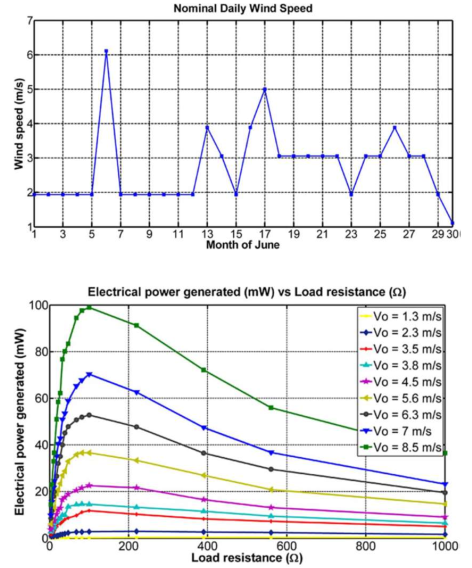
\includegraphics{images/windturbines.png}
      \caption{Wind turbines energy production diagram}
      \label{fig:windturbines}
   \end{figure}
\end{paracol}